\documentclass[conference]{IEEEtran}
\usepackage{textcomp}
\usepackage{lscape}
\usepackage{graphicx}
\usepackage{cite}
\usepackage{amsmath}
\usepackage{gensymb}
\usepackage[T1]{fontenc}
\title{ELEN4002: Digital Estimation of Body Mass Index}
\author{Darrion Singh (1056673)}

\begin{document}
\bstctlcite{IEEEexample:BSTcontrol}
\maketitle

\begin{abstract}
	
\end{abstract}

\section{Introduction}
The Body Mass Index (BMI) is a screening tool used to indicate whether one's body mass is healthy for their corresponding height \cite{nhsBMI}.
Whilst not an accurate diagnostic tool, the BMI provides a healthy body mass range for a particular height as it takes natural body shape variations into account \cite{nhsBMI}.
Unfortunately, the accurate collection of ones height and mass is time-consuming, especially when considering the time required to collect this data for large amounts of people.
Furthermore, the distance between rural areas and clinics also inhibit the habitants of the area from regular medical checkups, where a medical practitioner might require to measure and track ones height and mass.
A possible solution to both the above mentioned problems would be the creation of a tool that would provide a medical practitioner with this information without the need for the patient to be physically present.
The following report presents a study of a potential technique to estimate BMI from a photograph. It also reports on the design and implementation of program that estimates BMI from a photograph using these techniques, which include a mixture of Computer Vision and Machine Learning.
The School of Electrical and Information Engineering (EIE) have collaborated with the Peri-Natal HIV Research Unit (PHRU) for this project.
\section{Background}
\subsection{Project Concept}
The aim of this project is to estimate the BMI of a person from their photograph.
This is to be achieved by creating a program which accepts a front and side photograph of a person.
The program will extract body shape data from the photographs with the use of Computer Vision, and predict one's BMI based on their body shape data using Machine Learning.

The purpose of such a tool has vast applications in the medical field, whether it be used as a time-efficient means of tracking the progress of a disease/disorder that affects ones mass, or for a simple indication of ones own health.
Furthermore, a possible extension of this tool would be using it to classify which catergory of BMI one falls into: Underweight (< 18.5), Healthy (18.5 -- 25), Overweight (25 -- 30), or Obese (> 30).

The success of this project would result in the production of a BMI estimator which precludes the need for a subject to remove their clothes, as well as travel to a clinic for BMI measurement.
In large rural clinics, where large patient volumes combined with time taken to undress and redress for accurate height and mass measurements, this digital solution may result in a significant reduction in the time taken for consultations.
Furthermore, this solution would not be affected by measurement errors resulting from incorrect calibration of machinery.

\subsection{Assumptions \& Constraints}
\begin{itemize}
	\item As to provide the least chance of a false human body outline being detected, we assume that any person being photographed is staged in front of a uniform background, such as a wall whose colour significantly contrasts with that of the patient and their clothes.
	It is further assumed that all photographs used to train the machine learning algorithm should abide by the same assumption.
	\item In order to provide a measurement reference, the person in each photograph should be standing next to a reference object of known dimensions, such as a piece of standard A4 paper. The colour and dimensions of the piece of paper should be the same throughout the training dataset.
	\item This reference object is present in the photographs during any live testing or usage of the application.
	\item All subjects in the photographs stand alongside and in line with the reference object, i.e. if the reference object is stuck to a wall, the subject is standing against the wall.
	\item The distance between the camera and the subjects being photographed is constant and far enough away to capture the subject's full body photograph.
	\item Subjects have a maximum height of two meters.
	\item The time frame for this project is six weeks, with a total budget of R1200.
\end{itemize}

\subsection{Success Criteria}
\begin{itemize}
	\item The program should provide an average accuracy of 75\% for it to be classified as a potential viable solution.
	\item To be considered a working prototype, it should provide an average accuracy of 85\%.
	\item To be considered a completed product, it should provide a minimum average accuracy of 95\% across all age, gender, and mass groups.
	\item BMI prediction takes place without the need for one to remove their clothes and thus operate with pictures of clothed people.
	\item The final solution is a robust desktop application that can be easily used by a medical practitioner.
	\item The solution should be camera-independent and resolution-independent.
\end{itemize}

\subsection{Optional Criteria}
\begin{itemize}
	\item The software and it's trained neural network models are exported to either a mobile application or desktop executable. In this way, one could select a photograph from their cellphone/desktop gallery and the program could perform estimation on the chosen picture.
	\item The desktop executable can receive pictures from a connected camera.
	\item A mobile application would access the cellphone's camera and perform a BMI estimation from a photograph taken in-app. The prediction could either be shown to the user or sent to the medical practitioner directly.
	\item Provided that there is sufficient training data, training two separate models for male and female data points would decrease sex bias in the models. This would be to further improve accuracy by accounting for natural variations of body shape between men and women, with the hope of seeing similar statistical variations in BMI across age and sex as seen in Ref. \cite{bmiage}.
\end{itemize}

\section{Literature Review}
\subsection{Weight and Diameter Estimation}
Comert et al. aims to estimate the mass of an apple through image processing and machine learning techniques \cite{comert}.
The original apple image is seen as the top left image of Figure \ref{fig:segmentedapples}.
The process involves using the Prewitt edge extraction algorithm in order to obtain a binary image, seen as the top right image of Figure \ref{fig:segmentedapples}.
The binary image goes through Closing, filtering and Opening.

Closing is the process of performing Dilation followed by Erosion on an image, whilst Opening is the process of performing Erosion followed by Dilation on an image \cite{opening,closing}.
Dilation is a morphological operation whereby the value (intensity) of a pixel is increased to that of the pixel in its neighbourhood with the highest intensity \cite{mathworksdilationerosion}.
Erosion is a morphological operation whereby the value of a pixel is decreased to that of the pixel in its neighbourhood with the lowest intensity \cite{mathworksdilationerosion}.

This is done in order to improve the image quality for feature extraction, since Closing an image improves the prevalence of contours, whilst Opening an image improves the uniformity of the spaces between contours.
The bottom image of Figure \ref{fig:segmentedapples} shows the binary image after the above operations were performed on it, successfully segmenting the pixels of the apple as white whilst the background is black.

\begin{figure}
    \centering
    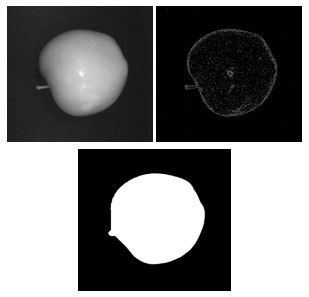
\includegraphics[width=0.7\linewidth]{segmentedapples.jpg}
    \caption{Segmentation techniques to isolate the apple in the image \cite{comert}.}
    \label{fig:segmentedapples}
\end{figure}

Feature extraction is carried out such that the area and diameter of the apple are extracted seen in Figure \ref{fig:diameterapples}.
This feature extraction would then be performed on a set of apple photographs whose masses were known.
Thereafter, the diameter and area of the apples were related to their recorded masses using a linear regression model.
This method reported a 96.5\% accuracy of estimation \cite{comert}.

\begin{figure}
    \centering
    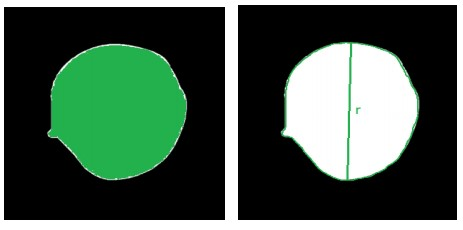
\includegraphics[width=0.7\linewidth]{diameterapples.jpg}
    \caption{Apple Area and Diameter Extraction  \cite{comert}.}
    \label{fig:diameterapples}
\end{figure}

\subsection{Weight Estimation Using Image Analysis and Statistical Modelling}
Similar to the requirements of the BMI system, Kollis et al. discusses a robust image analysis based mass estimation of pigs in large scale livestock farming \cite{kollis2007weight}. 
The software of choice for image processing is MATLAB in which the Image Processing Toolbox V4.1 is used.
Object detection occurred through comparison between the camera environment without the pig and with the pig.
This results in a binary image that undergoes segmentation, filtering and opening to get a clear image for feature extraction.

Feature extraction in this paper is particularly relevant to this report as the body shape of the pigs is more complex than the features of apples described by Ref. \cite{comert} in the previous section. 
The feature extraction method is comprised of the skeletonisation function in MATLAB which generates a skeletal structure of the object in question.

Figure \ref{fig:pigskeleton} shows the skeletonisation process for the image of the pig.
\begin{figure}
    \centering
    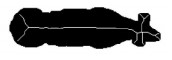
\includegraphics[width=\linewidth]{pigskeleton.jpg}
    \caption{Skeletonisation function implemented on pig binary image\cite{kollis2007weight}.}
    \label{fig:pigskeleton}
\end{figure}

Using this process the spine (main branch) is used to estimate the length of the pig by counting the pixels which comprise the spine.
Thereafter, the estimated spine length and recorded pig masses were related using a linear regression model.

\subsection{Human Weight from a RGB-D Image}
Nguyen et al. explores human mass prediction through a single RGB-D image \cite{nguyen2014seeing}.
The camera in question uses a depth sensor to create a separate depth image. 
This extra image proves to be useful in object detection due to depth allowing an accurate trace of the human body shape with the aid of the 2D RGB image. 

This silhouette is passed through similar image processing methods used in the aforementioned papers. 
However, mass prediction is different in this scenario as the author used various mathematical relationships relating body width, height and area with Support Vector Regression to predict the mass of the person through the extracted features.

\subsection{Types of Neural Networks}
Mehta discusses the various types of neural networks and what applications in which they prove to be useful \cite{mehta_2019}. 
The summary is as follows:
Feed-Forward neural networks were useful in situations with minimal data-sets, as well as data-sets that have a substantial amount of noise.
The multi-layer perceptron is used when the training data-set is not linearly separable.
Networks that make use of back propagation need large data-sets and is generally used in when the network needs to recall or retain information.
Convolutional neural networks are used in applications such as object detection and image classification.

\subsection{Estimation of BMI from Photographs Using Deep Convolutional Neural Networks}
Pantanowitz et al. have conducted a similar undertaking to that described in this report.
The paper discusses the estimation of BMI from a photograph using a Deep Convolutional Neural Network \cite{bmifromphoto}.
The analysis was performed on a dataset of 161 photographs that were used to create a set of silhouette images via manual marking as well as automated image processing techniques.
The silhouette images were standardised to a particular pixel width without changing aspect ratio, and were theereafter padded appropriately and cropped to a square bounding box.
The silhouette images were augmented via minimal rotations and width shifts, with the author stating that the model could only train sufficiently with augmentation.
A rather complicated model consisting of 17 layers was used, details of which can be found in Ref. \cite{bmifromphoto}.
The results showed the BMI predictions having a correlation of 0.96 with the actual BMI values.

\section{System Design}
The proposed solution comprises of two subsystems, namely the Extraction layer and the Machine Learning layer.
These subsystems have no dependency on each other and are to be built independently of one another.
Figure \ref{fig:systemblockdiagram} in Appendix 5 provides a system diagram showing the inputs and outputs of each system, as well as the components of each system.
The Extraction layer comprises of the Object Detection, Image Segmentation and Input Extraction components, whilst the Machine Learning layer comprises of the Front View, Side View and Weighted Averaging components.
\subsection{Extraction Layer}
A front and side view photograph of a person with the aforementioned reference object in the top left corner is the input into the system.
For the sake of clarity and simplicity, the reference object chosen is a standard A3 cardboard, and its chosen colour is black for the sake of high contrast with the assumed light coloured wall in the background.
The Object Detection component will isolate the two objects in the photograph, namely the person and the reference object, and return the bounding box for each.
The width of the bounding box surrounding the reference object is measured in pixels.
Knowing its physical width allows us to calculate the pixels per meter ratio for that photograph.
In other words, all objects that exist in line with the reference object will be represented by approximately the same number of pixels per meter as that object.
This technique was inspired by Ref. \cite{objectDetection}.

For both the front and side view photographs the Image Segmentation component will receive the locations of the reference object and the person in the form of their bounding boxes.
Using the bounding boxes, both the reference object's and person's pixel mask (all pixels belonging to an object) will be extracted for both the front and side photographs.

Using the pixels per meter found earlier the Input Extraction component performs feature extraction on the person's front and side pixel masks.
Six features are extracted from each pixel mask:
\begin{itemize}
	\item Their approximate height in meters.
	\item The approximate two dimensional area contained within their shape (silhouette) in squared meters.
	\item The maximum thickness of their thoracic region in meters.
	\item The maximum thickness of their abdominal region in meters.
	\item The maximum thickness of their pelvic region in meters.
	\item The maximum thickness of their upper leg region (thigh) in meters.	
\end{itemize}
Note that from front images, the 'thickness' is hereafter referred to as 'width' whilst from the side images, 'thickness' is hereafter referred to as 'depth'.
The four body regions mentioned above have been chosen strategically as to represent common areas of body fat deposit. %*************************FIND REFERENCE*************************************************
In other words, this study explores the use of Computer Vision and Machine Learning to relate the common regions of body fat deposit to BMI by extracting information about these regions from photographs.
The output of the Extraction layer is two vectors, namely the front view vector (FVV) and side view vector (SVV).
Both FVV and SVV will contain the above mentioned features extracted from their respective photograph.

\subsection{Machine Learning Layer}
All the outputs of the Extraction layer mentioned above are provided as inputs into the Machine Learning layer.
The FVV and SVV are passed into the Front View and Side View components respectively, both of which are neural network models trained on a dataset of FVV's and SVV's, respectively.
Both networks will have been trained to estimate BMI independently until an acceptable accuracy is achieved, or falling short of that, the best possible accuracy is achieved.

The estimated BMI from the Front View and Side View component are then used as inputs into a final neural network, the Error Correction / Compensation component, which performs a weighted averaging between the Front and Side BMI estimations.
This network will have been trained to estimate BMI by deciding the contribution that the Front and Side view estimates should make towards a final BMI estimation with improved accuracy.
\section{Training Data Collection}
\subsection{Ethics Approval}
\subsection{Collaboration with the PHRU}
The PHRU have provided clinical research staff
\subsection{Data Types}
The data to be collected are as follows:
\begin{itemize}
\item A front and side photograph of the subject.
Both photographs should have the reference object in the top left corner of the image.
As mentioned above, the background of the image should be a uniform surface such as a wall.
This is to ensure that the image pre-processing techniques described in the succeeding sections of this report can be carried out without error.
\item The height and mass of each person.
These must be captured simultaneously and attached to the front and side photographs.
Data survey applications such as \textit{REDCap} may be useful in achieving this.
\item (Optional) Sex of person in each photograph.
Whilst this characteristic is not an input into the system, it should be recorded for statistical purposes for later quantification of algorithmic bias.
Furthermore, to achieve the optional criteria discussed above, data points must be labelled as male/female to train separate models.
\item (Optional) Race of person in each photograph.
This characteristic could also be recorded for statistical purposes.
Furthermore, it opens an avenue for further research into how ethnicity can be used to narrow BMI distribution and hence provide more accurate BMI estimations.
\item (Optional) Age of person in each photograph.
This characteristic, despite only being recorded for statistical purposes, is by far the largest contributor to the distribution of BMI, as seen in Ref. \cite{bmiage}.
Knowing the distribution of the age of the subjects will provide a range of ages where the program is likely to provide the most accurate estimation.
\end{itemize}
With the ultimate aim in mind for this program to be a universal BMI estimator, it is encouraged that the data-set of subjects who volunteer to be photographed be spread in terms of sex, ethnicity and age.
\subsection{Obtaining Data}
It is possible to find such images of people on the internet, however it is unlikely for these images to have the corresponding height and mass on record.
The chosen method for obtaining the data is to illicit the help of a medical research group who have access to large amounts of people, along with properly calibrated height and mass measuring equipment.

It should be noted that obtaining data in this manner requires prior clearance from a recognised ethics committee, as well as the permission of those in charge of the proposed sites such as research clinics.
As with most neural network related projects, it is encouraged for a large data-set to be collected, and it was decided that a reasonable minimum number of subjects would be 100.



\section{Methodology}

\section{Sources of Error}

\section{Findings \& Analysis}

\section{Additional Features}

\section{Recommendations}

\section{Conclusion}

\section{Acknowledgements}

\bibliographystyle{IEEEtran}
\bibliography{references}
\end{document}

%% paralax error because side photos have the side of people in front of the ref object